
\section{Prepare data}
\label{sec:dataPrepare}
\subsection{Raw data}

Data should be prepared as the example in Figure~\ref{fig:dataMicroarray}.
First column should be feature ID (e.g. gene symbol) and the rest of the columns are samples.
The first row is sample ID.
Valid data type includes continuous, count.

\begin{figure}[H]
\begin{center}
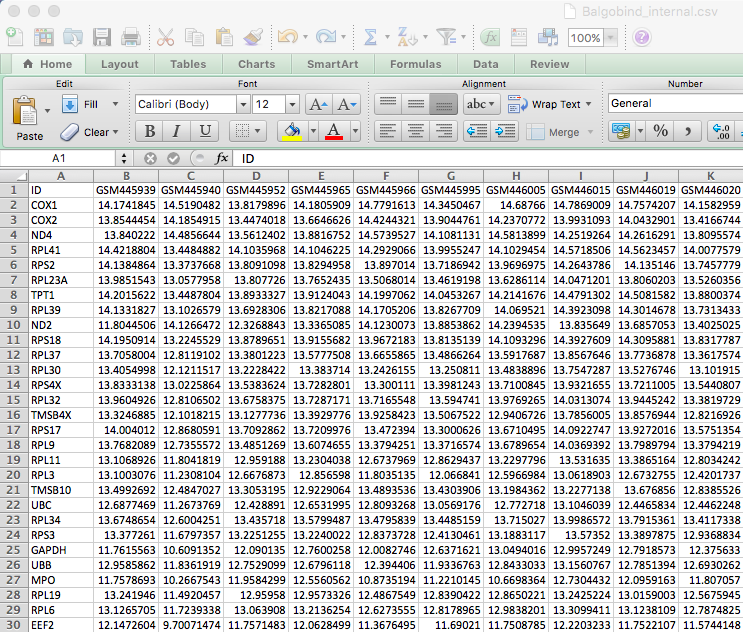
\includegraphics[scale=0.5]{./figure/dataMicroarray}
\caption{A example data format}
\label{fig:dataMicroarray}
\end{center}
\end{figure}

\subsection{Clinical data}

Clinical data should be prepared as the example in Figure~\ref{fig:clinical}.
First column should be sample ID and each row represents a sample.
The rest of the columns are clinical information.

\begin{figure}[H]
\begin{center}
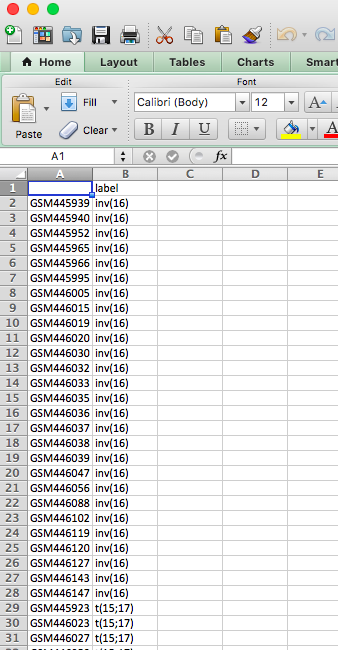
\includegraphics[scale=0.5]{./figure/clinicalData}
\caption{A example clinical data format}
\label{fig:clinical}
\end{center}
\end{figure}
